\section{匀速运动与直线} \label{sec:curve-line}

匀速运动是速度(向量)保持不变的运动,
设$t=0$时刻的位置为$\vec r_0$,
速度保持为$\vec v_0$, 则点在$t$时刻的位置为
$\vec r(t) = \vec r_0 + \vec v_0 t$,
运动的轨迹是一条直线.
匀速运动是非常简单的一类运动, 相信读者早已非常了解了,
我也没有什么能介绍的内容. 所以我们主要探讨一下直线的各种方程.

\hlinefill

\noindent $x=x_0$和$y=y_0$ ($x_0,y_0$为定值)

水平线和竖直线有非常简单的方程. 一条水平线上所有点的纵坐标都相同,
设为$y_0$, 那么$y=y_0$就是该水平线的方程. 竖直线$x=x_0$同理.

\hlinefill

\noindent $y=kx+b$ ($k,b$为定值)

这是初中数学常用的直线方程, 核心是$y$和$x$的函数关系:
$y$随$x$变化的变化率保持不变.
$k$对应$y$随$x$的变化率, 反映了直线的倾斜程度, 被称为直线的\emph{斜率}.
如图\ref{fig:line-k}, 斜率$k$的绝对值越大, 直线越接近竖直线.
设直线的倾斜角为$\alpha$ (水平线的倾斜角为$0\degree$),
则有$k = \tan\alpha$.
$b$对应直线与$y$轴交点的纵坐标, 反映了直线的整体位置,
被称为直线的\emph{截距}.

\begin{figure}[htbp]
  \centering
  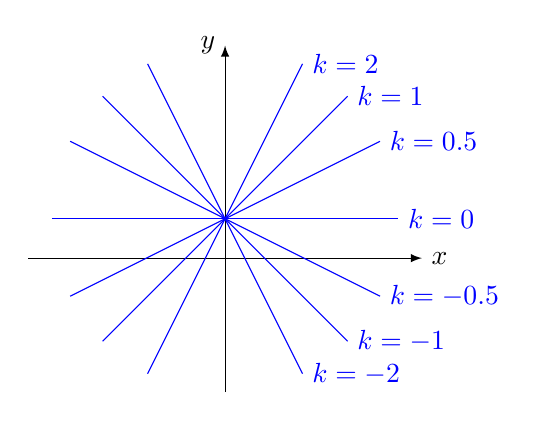
\begin{tikzpicture}
    \draw[-latex] (-2.5,0) -- (2.5,0) node[right] {$x$};
    \draw[-latex] (0,-1.7) -- (0,2.7) node[left] {$y$};
    \begin{scope}[yshift=0.5cm]
      \foreach \k in {-2,-1,-0.5,0,0.5,1,2}
      \draw[blue] ({atan(\k)}:-2.2) -- ({atan(\k)}:2.2)
      node[right] {$k=\k$};
    \end{scope}
  \end{tikzpicture}
  \caption{直线的斜率 ($y=kx+1$)}
  \label{fig:line-k}
\end{figure}

作为一个函数形式的方程, 它的实用性还挺不错的,
但是它有一个比较大的缺点: 不能表示竖直线.
虽然我们可以用分类讨论来弥补这一点,
但是和后面介绍的方程相比它就基本没有什么优势了.

\hlinefill

\noindent $ax+by+c=0$ ($a,b,c$为定值, $a,b$不同时为0)

这是高中数学常用的直线方程, 可以描述平面上的任意直线.
作为一般方程, 它非常符合高中的解析几何的风格, 理论意义很大,
但在弹幕制作上的应用基本没有. 所以我们直接看下一个.

\hlinefill

\noindent $\vec r=\vec r_0+\vec v_0\cdot t$
($\vec r_0,\vec v_0$为定值)

\noindent 坐标形式: $\begin{cases}
    x=x_0+v_{x0}\cdot t \\ y=y_0+v_{y0}\cdot t
  \end{cases}$

这是由平面上的匀速运动得到的参数方程.
$\vec r_0=(x_0,y_0)$是直线上的一点,
$\vec v_0=(v_{x0},v_{y0})$决定了直线的朝向.
我们将$\vec v_0$称为直线的\emph{方向向量}.
这是直线的一个基本的参数方程, 接下来我们会看到一些针对特定需求的改写形式.

将参数$t$的范围加以限制, 还可以构造直线的一部分.
比如限制$t\ge0$, 就可以得到以$\vec r_0$为端点,
$\vec v_0$方向的射线.

\hlinefill

\noindent $\vec r=\vec r_0+\braket{t,\alpha}$
($\vec r_0,\alpha$为定值)

\noindent 坐标形式: $\begin{cases}
  x=x_0+t\cos\alpha \\ y=y_0+t\sin\alpha
\end{cases}$

该方程描述了一条经过点$\vec r_0=(x_0,y_0)$, 倾斜角为$\alpha$的直线.
它使用$(\cos\alpha,\sin\alpha)$作为方向向量,
直接把直线的倾斜角和方程联系在一起,
并且, 参数$t$直接对应直线上的点与$\vec r_0$的距离.

\begin{center}
  \begin{tikzpicture}
    \draw (0,0) -- (10:5);
    \node[dot,label={above:$\vec r_0$}] at (10:2) {};
    \draw[->] (4,0.3) -- +(10:4mm) node[right] {$\alpha$};
    \foreach \t in {-1,1,2}
    \node[dot,label={above:$t=\t$}] at (10:{2+\t*1.2}) {};
  \end{tikzpicture}
\end{center}

\hlinefill

\noindent $\vec r=\vec r_1+(\vec r_2-\vec r_1)t$
($\vec r_1,\vec r_2$为定值)

\noindent 坐标形式: $\begin{cases}
  x=x_1+(x_2-x_1)t \\ y=y_1+(y_2-y_1)t
\end{cases}$

该方程描述了一条经过点$\vec r_1=(x_1,y_1)$和$\vec r_2=(x_2,y_2)$的直线,
与\ref{sec:vec-calc}节提到的线性插值问题相照应.

如果限制$0\le{t}\le1$, 可以得到以$\vec r_1,\vec r_2$为端点的线段.

\hlinefill

最后顺便说一说正多边形. 虽然我们可以在网上搜索到正多边形的方程
(多半是极坐标方程), 但分段构造线段方程仍然是更好的方法,
比起强行代入正多边形方程, 分段构造的可读性高, 更加自由,
同时实现起来也并不复杂, 而且很容易扩展到一般的折线.
下面是一个基于五角星的风车弹幕, 读者可以自行尝试.

\begin{center}
  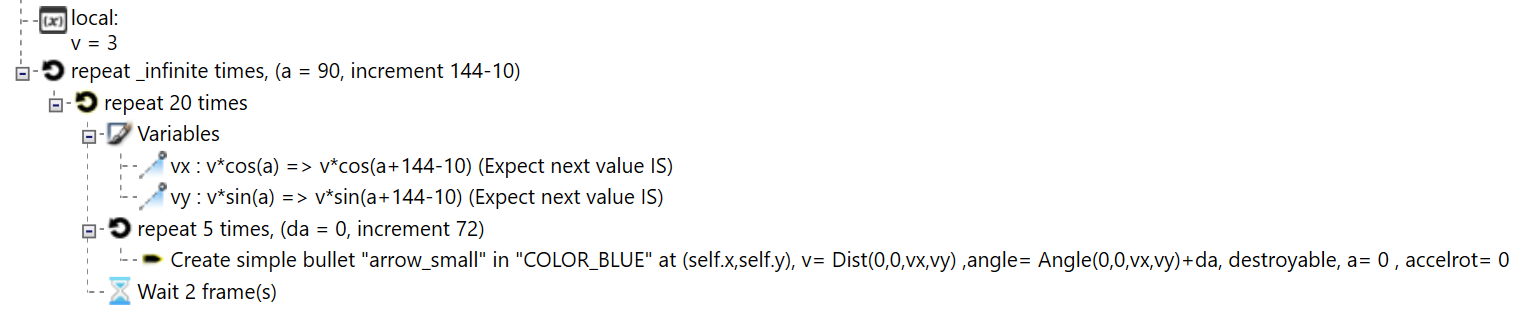
\includegraphics[width=\textwidth]{assets/curve/star-code.png}
\end{center}
